\documentclass[crop,tikz]{standalone} 
\usepackage{tikz, amsmath, amssymb, graphicx} 

\DeclareMathAlphabet\mathbfcal{OMS}{cmsy}{b}{n}

\newcommand{\Mt}{\mathbfcal{M}}
\newcommand{\Yt}{\mathbfcal{Y}}
\newcommand{\Ft}{\mathbfcal{F}}

\usetikzlibrary{positioning, shapes.geometric} 

\begin{document} 

\begin{tikzpicture} 


\node[inner sep=0pt] (sim:0.05) at (0,0) {
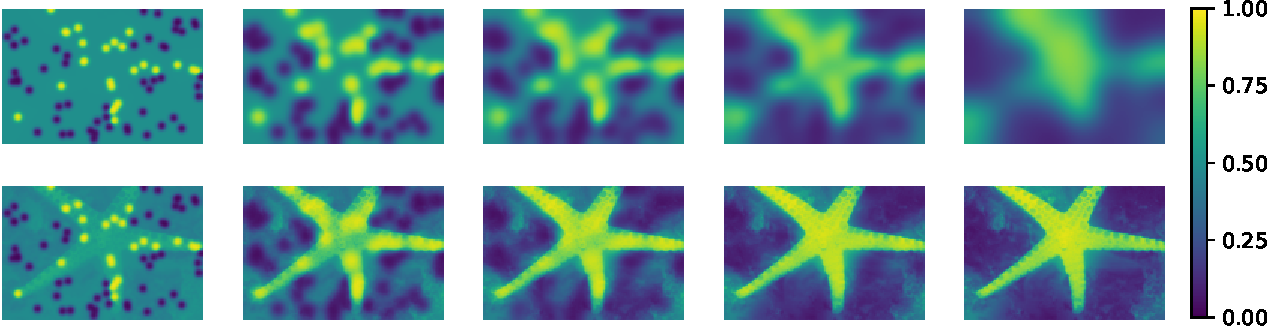
\includegraphics[width=\textwidth]{starfish2.pdf}
}; 
  


\draw (-5.0, 1.8) node {$\beta=10$};
\draw (-2.7, 1.8) node {$\beta=50$};
\draw (-0.4, 1.8) node {$\beta=100$};
\draw (1.9, 1.8) node {$\beta=200$};
\draw (4.2, 1.8) node {$\beta=500$};


\draw (-7, 0.85) node {L-GSR};
\draw (-7, -0.85) node {L-RNC};


% \draw (6.8,2.7) node {CGM};

% \draw (-4.2,0.3) node {$m=0.05$};
% \draw (-4.2,-4.7) node {$m=0.5$};
% \draw (-4.2,-9.7) node {$m=0.95$};


\end{tikzpicture}
\end{document} 
